\documentclass{standalone}
\usepackage{tkz-base}
\usepackage{tkz-fct}
\usepackage{tkz-euclide}
\usepackage{tikz}
\begin{document}
    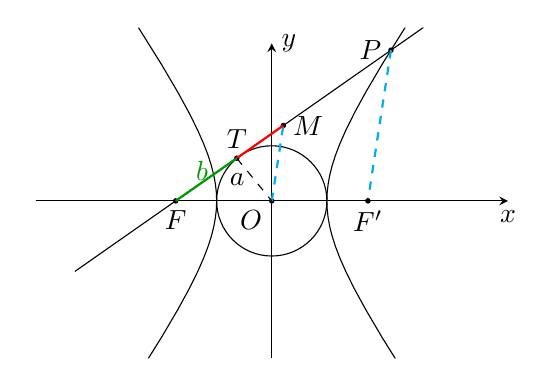
\begin{tikzpicture}
        \pgfmathsetmacro\xx{3}
        \pgfmathsetmacro\y{2}
        \pgfmathsetmacro\a{0.7}
        \pgfmathsetmacro\b{1}
        \pgfmathsetmacro\c{sqrt(abs(\a^2+\b^2))}
        \pgfmathsetmacro\px{1.3}
        \pgfmathsetmacro\py{sqrt(-1*\b^2*(1-(\px^2)/\a^2))}
        \coordinate (O) at (0,0);
        \coordinate (F1) at (-\c,0);
        \coordinate (F2) at (\c,0);
        \coordinate (P) at (\px,\py);
        \tkzInit[ymax=\y,ymin=-\y,xmax=\xx,xmin=-\xx] 
        \clip (-\xx-0.1,0) |- (0,\y+0.2) -| (\xx+0.2,0) |- (0,-\y) -| cycle;
        % \tkzFctPar[samples=400,domain=-0.4*pi:0.4*pi]{\a/(cos(t))}{\b*(tan(t))}
        % \tkzFctPar[samples=400,domain=0.6*pi:1.4*pi,name path = a]{\a/(cos(t))}{\b*(tan(t))}
        \draw [domain = -0.4*pi:0.4*pi,name path = a] plot ({\a/(cos(\x r))},{\b*(tan(\x r))});
        \draw [domain = -0.4*pi:0.4*pi] plot ({-\a/(cos(\x r))},{\b*(tan(\x r))});
        \draw [domain=-2.5:3,name path= b]plot (\x,{0.7*(\x+\c)});
        \fill [name intersections={of=a and b,by={A}}]
        (A) circle (1pt) node [left] {$P$};
        \coordinate (M) at ($(A)!0.5!(F1)$);
        \draw[cyan,thick,dashed] (A) -- (F2);
        \draw[name path =c] (O) circle (\a);
        \fill [name intersections={of=c and b,by={T}}]
        (T) circle (1pt) node [above] {$T$};
        \draw[-stealth] (-\xx,0) -- (\xx,0) node [below] {$x$};
        \draw[-stealth] (0,-\y) -- (0,\y) node [right] {$y$};
        \fill (O) node [below left] {$O$} circle (1pt);
        \fill (F1) node [below] {$F$} circle (1pt);
        \fill (F2) node [below] {$F'$} circle (1pt);
        \fill (M) node [right] {$M$} circle (1pt);
        \draw[cyan,thick,dashed] (O)--(M);
        \draw[red,thick] (T)--(M);
        \draw[dashed] (T)--(O) node[pos=0.5,left]{$a$};
        \draw[thick,green!60!black] (T)--(F1) node[pos=0.3,left]{$b$};
    \end{tikzpicture}
\end{document}